\chapter{Конструкторский раздел}
\section{Схемы алгоритмов Левенштейна}
Ниже представлены следующие схемы алгоритмов:
\begin{itemize}
	\item рис. \ref{png:1} - схема алгоритма итеративного Левенштейна с использованием двух строк;
	\item рис. \ref{png:2} - схема алгоритма рекурсивного Левенштейна без кэша;
	\item рис. \ref{png:3} и рис. \ref{png:4} - схема алгоритма рекурсивного Левенштейна с использованием матрицы;
	\item рис. \ref{png:5} - схема алгоритма рекурсивного Дамерау-Левенштейна.
\end{itemize}

\begin{figure}[pht!]
	\centering{
		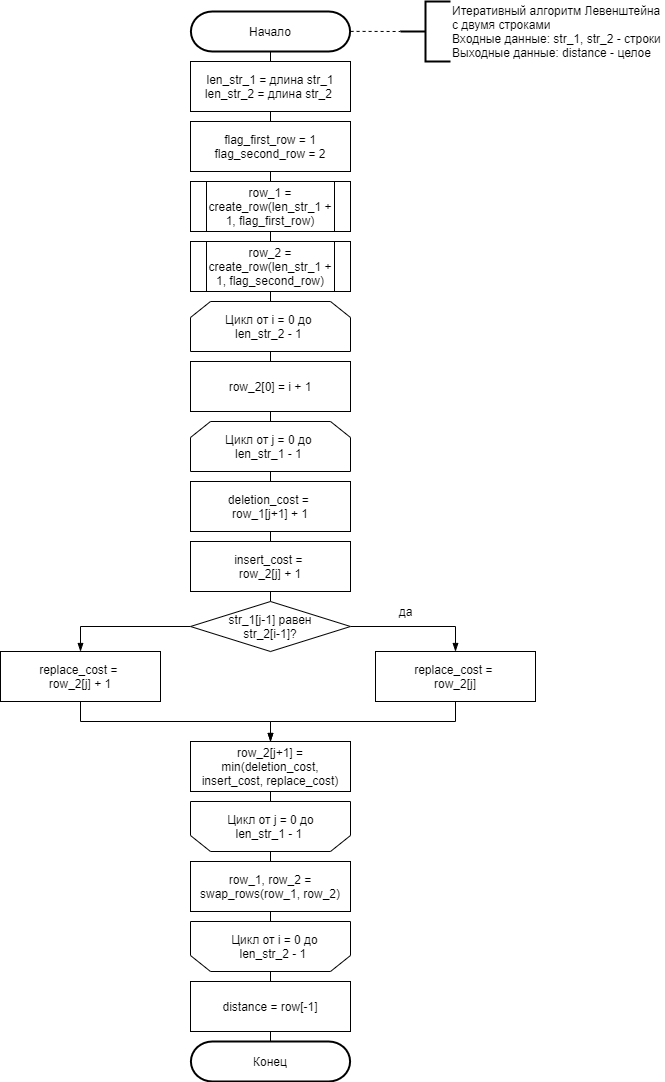
\includegraphics[width=14.6cm]{../../../../../../../msys64/home/Лев/bmstu_sem_5_aa/lab_01/report/diagrams/iterative_two_rows}
		\caption{Ссхема алгоритма итеративного Левенштейна с использованием двух строк.}
		\label{png:1}}
\end{figure} 

\begin{figure}[pht!]
	\centering{
		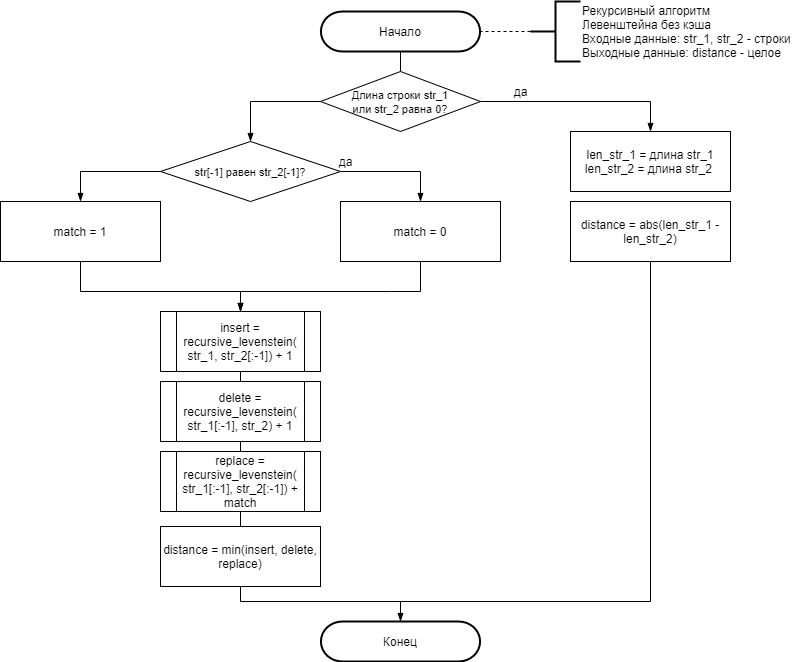
\includegraphics[width=14.6cm]{../../../../../../../msys64/home/Лев/bmstu_sem_5_aa/lab_01/report/diagrams/Рекурсивный Левенштейн без кэша}
		\caption{Схема алгоритма рекурсивного Левенштейна без кэша.}
		\label{png:2}}
\end{figure} 

\begin{figure}[pht!]
	\centering{
		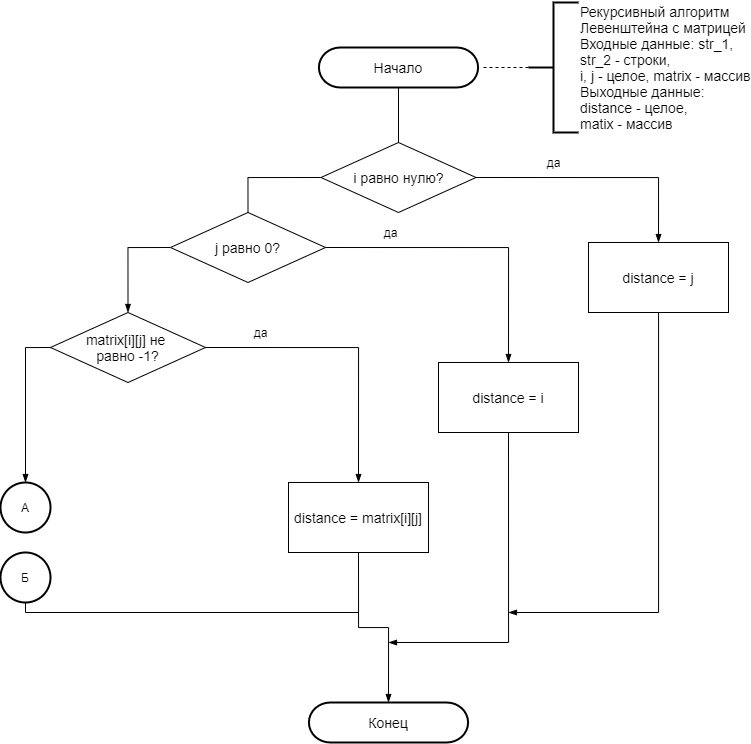
\includegraphics[width=14.6cm]{../../../../../../../msys64/home/Лев/bmstu_sem_5_aa/lab_01/report/diagrams/Рекурсивный Левенштейн с матрицей1}
		\caption{Cхема алгоритма рекурсивного Левенштейна с использованием матрицы.}
		\label{png:3}}
\end{figure}

\begin{figure}[pht!]
	\centering{
		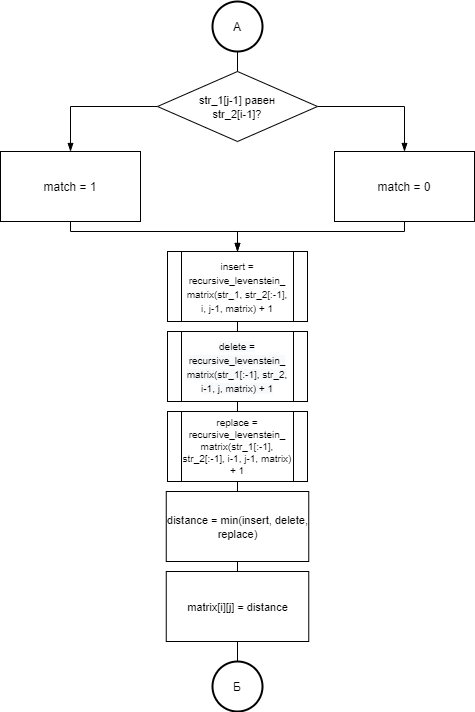
\includegraphics[width=14.6cm]{../../../../../../../msys64/home/Лев/bmstu_sem_5_aa/lab_01/report/diagrams/Рекурсивный Левенштейн с матрицей2}
		\caption{Схема алгоритма рекурсивного Левенштейна с использованием матрицы.}
		\label{png:4}}
\end{figure}  
\newpage

\begin{figure}[pht!]
	\centering{
		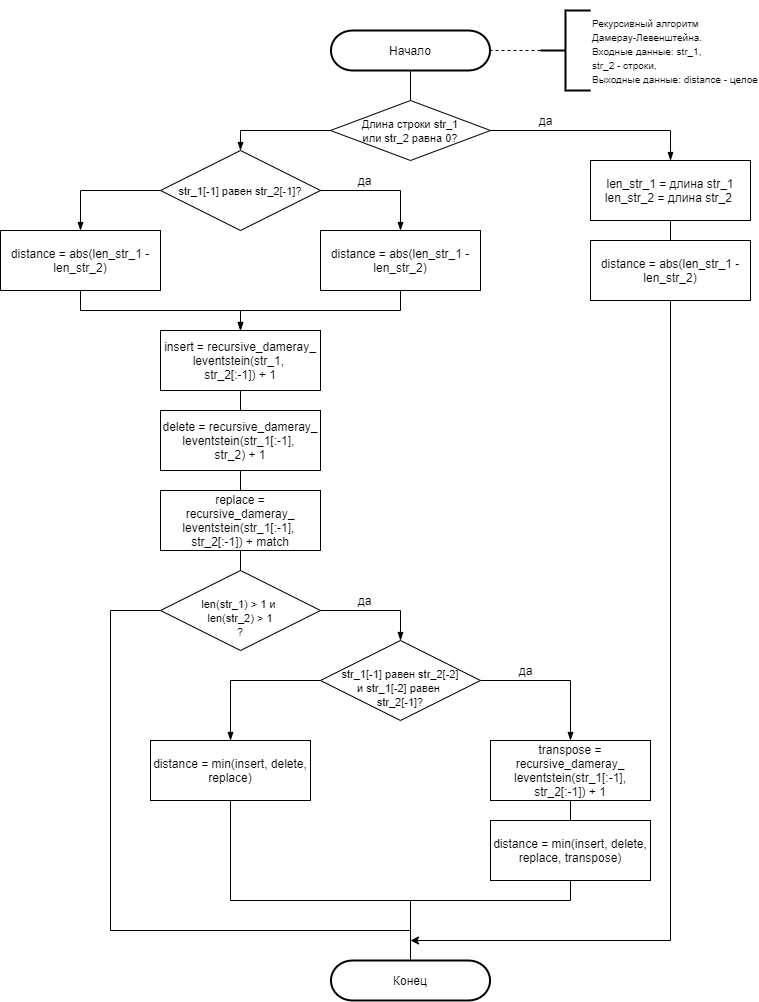
\includegraphics[width=14.6cm]{../../../../../../../msys64/home/Лев/bmstu_sem_5_aa/lab_01/report/diagrams/Рекурсивный Дамерау-Левенштейн}
		\caption{Схема алгоритма рекурсивного Дамерау-Левенштейна.}
		\label{png:5}}
\end{figure}

\section*{Вывод}
На основе теоретических данных, полученных в аналатическом разделе, были построены схемы нужных алгоритмов.